\subsection{实验目的}
进一步学习雷达信号处理中的线性调频信号及其脉冲压缩技术,分析非基带信号的脉冲压缩结果,窗效应,以及基带信号中的失配影响。
\subsection{实验原理}
\subsubsection{非基带信号的脉冲压缩}
\paragraph{非基带信号}
在时域中,非基带信号可以视为零频率时刻偏离脉冲中心的信号。设$t_c$是脉冲中心相对于$t=0$的时间偏移,则发射信号为
\begin{equation}
s(t) = \rectf{\frac{t}{T}}\exp(\jj\pi\gamma(t-t_c)^2)
\end{equation}
回波信号
\begin{equation}
s_r(t)=\rectf{\frac{t-t_0}{T}}\exp(\jj\pi\gamma(t-t_0-tc)^2)
\end{equation}
滤波器冲击相应函数
\begin{equation}
h(t)=s^*(-t)=\rectf{\frac{t}{T}}\exp\left(-\jj\pi\gamma(t+t_c)^2\right)
\end{equation}
匹配滤波器输出
\begin{equation}
s_{out}(t)=T\exp(-\jj2\pi\gamma t_c(t-t_0))\sinc(\gamma T(t-t_0))
\end{equation}
\subsubsection{点目标的质量参数}
点目标在处理后的SAR图像中表现为sinc型函数。点目标测量给出的重要的质量参数包括:
\begin{description}
	\item[冲击相应宽度(IRW)] 冲击响应的3dB主瓣宽度。冲击响应是输入为冲击函数时的系统输出。在SAR系统中,它是通过测量地面的一个单一鼓励散射体的系统响应得到的。
	\item[峰值旁瓣比(PSLR)] 最大旁瓣与主瓣的高度比,以分贝表示。sinc函数的PSLR为-13dB。SAR系统中的PSLR必须小于该值,以是的弱目标不会被邻近的强目标掩盖。PSLR一般取在-20dB左右。可以通过使用窗函数达到这一要求。
	\item[一维积分旁瓣比(ISLR)] 对冲击响应功率(幅度平方)进行积分得到。令$P_{main}$为主瓣功率,$P_{total}$为总功率,则一维$ISLR$为
	\[ ISLR=10\log_{10}\left( \frac{P_{total}-P_{main}}{P_{main}} \right) \]
	其中分子是旁瓣的总能量。主瓣宽度以峰值为中心,大小取为IRW的2-2.5被。也可以将相邻零点作为主瓣宽度,此时典型一维ISLR为-17dB。
\end{description}
\subsubsection{窗效应}
频谱近似为矩形时的PSLR为-13dB。一般认为这一PSLR过高,会淹没附近的弱目标。降低PSLR的一种方法是对频域匹配滤波器引入平滑窗,以减少主瓣到旁瓣的能量泄漏。

窗是一个对信号频谱进行加权的对称实函数。权值在信号频谱中心处最大,向频谱两边逐渐衰落。

窗能够平滑频谱,即弱化频谱边缘处的不连续性。这样会降低压缩脉冲中主瓣能量泄漏,但是会损失分辨率。因为窗是的压缩中的有效信号带宽变窄。
\paragraph{Kaiser窗}
有一个可调参数$\beta$,可以在不同应用中兼顾分辨率和旁瓣。

在时域中,长度为$T$的Kasier窗可以表示为
\begin{equation}
w_k(t, T) = \frac{I_0(\beta\sqrt{1-(2t/T)^2})}{I_0(\beta)},\quad -\frac{T}{2}\leq t\leq \frac{T}{2}
\end{equation}
其中$I_0$为零阶贝塞尔函数,$\beta$为可调整的衰减系数或平滑系数。

频域中,长度为$F$的Kasier窗可以表示为
\begin{equation}
W_k(f, F) = \frac{I_0(\beta\sqrt{1 - (2f/F)^2})}{I_0(\beta)}, \quad -\frac{F}{2}\leq f\leq\frac{F}{2}
\end{equation}
加权后的频域匹配滤波器
\begin{eqnarray}
H(f) = W_k(f, \abs{\gamma}T)\exp\left(\jj\pi\frac{f^2}{\gamma}\right)
\end{eqnarray}
加权后的时域匹配滤波器
\begin{equation}
h(t) = w_k(t, T)\exp(-\jj\pi\gamma t^2)
\end{equation}
输出信号
\begin{eqnarray}
S_{out}(f) &=& S_r(f)H(f) = W_k(f, \abs{K}T)\exp(-\jj2\pi ft_0) \\
s_{out}(t) &=& p(t - t_0)
\end{eqnarray}
\paragraph{展宽}
定义为加窗前后3dB宽度的比值。

分析不同$\beta$值时的Kaiser窗的PSLR以及相对于矩形窗的IRW展宽。$\beta$的一个典型值是2.5,与矩形窗相比,PSLR降至-21dB,分辨率扩展了1.18倍。
\subsubsection{基带信号中的失配影响}
一般用三个参数对线性调频信号的匹配滤波器加权加以描述,即持续时间、中心频率和调频率。其中,调频率的误差影响最严重。

通过对$H(f)$引入调频率wuia$\Delta K$,运用实验分析其影响。分析IRW,PSLR以及随二次相位误差QPE的变化。
\paragraph{QPE的定义}
当存在$\Delta K$时,信号与滤波器之间存在一个相位误差。设匹配滤波器的带宽与信号相同。忽略可能存在的常数相位偏移,假设匹配滤波器的中间相位与信号中间的相位匹配,则QPE为信号任意一端处的相对相位失配,此处失配最大。在此定义下,线性调频信号的QPE为
\[ QPE=\pi\Delta\gamma\left(\frac{T}{2}\right)^2 \]
\subsection{实验流程}
\begin{figure}[H]
	\centering
	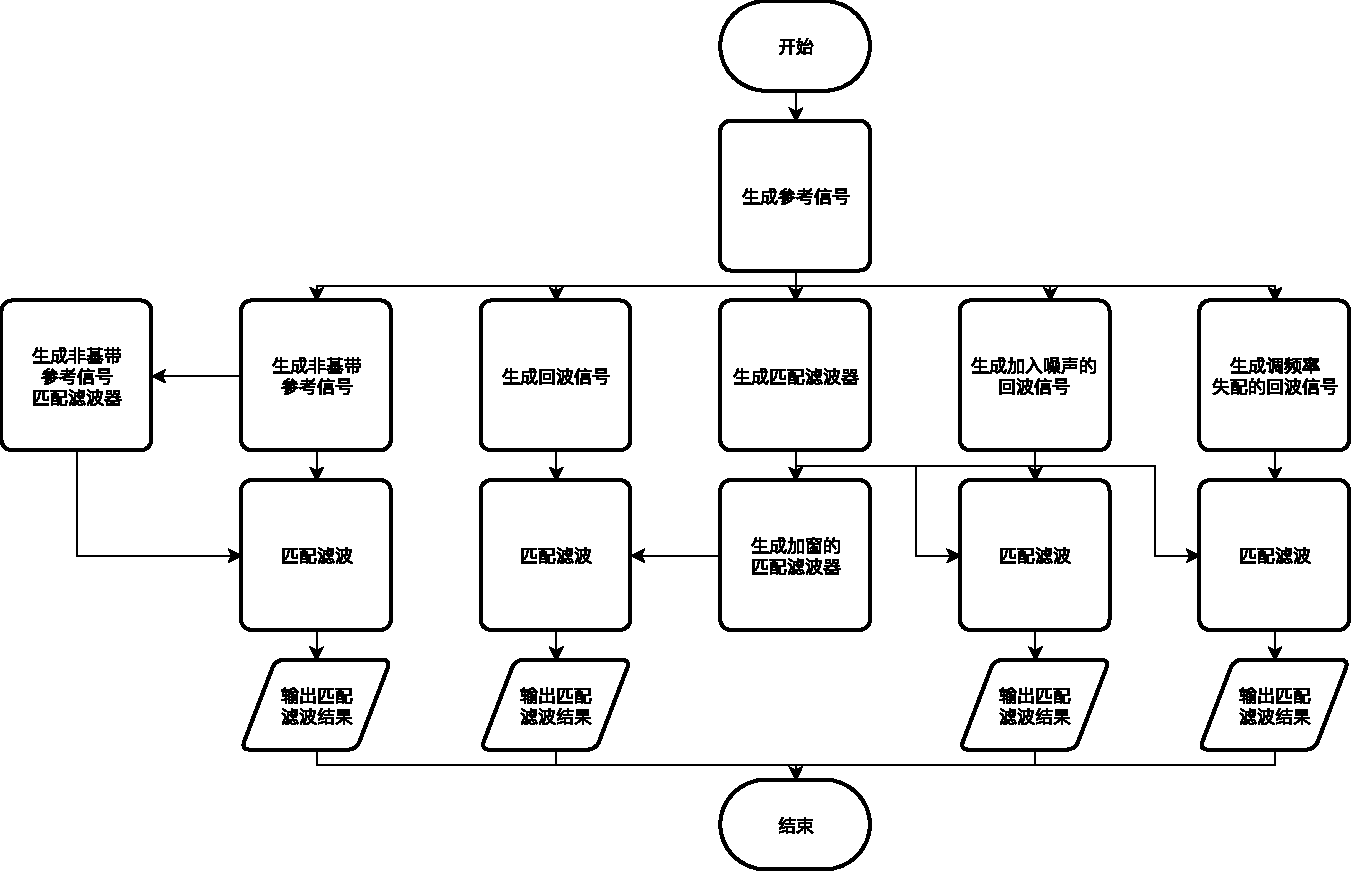
\includegraphics[width=\linewidth]{figure/AdvancedPulseCompressionFlowchart.pdf}
	\caption{脉冲压缩流程图}
\end{figure}
\subsection{实验程序}
\lstinputlisting[caption={非基带信号脉冲压缩}]{"../Executable Script/Exp 12/NoneBasebandPulseCompression.m"}
\lstinputlisting[caption={有噪声的脉冲压缩}]{"../Executable Script/Exp 12/NoisyPulseCompression.m"}
\lstinputlisting[caption={加窗的脉冲压缩}]{"../Executable Script/Exp 12/WindowedPulseCompression.m"}
\lstinputlisting[caption={调频率失配的脉冲压缩}]{"../Executable Script/Exp 12/MissingGammaPulseCompression.m"}
\subsection{实验结果和分析}
设定发射信号是100MHz带宽, 10$\mu$时宽的线性调频信号,回波信号在17$\mu$s后返回。对回波信号进行不同的处理,得到不同的结果。
\subsubsection{非基带信号的脉冲压缩}
\begin{figure}[H]
	\centering
	\begin{minipage}{0.45\linewidth}
		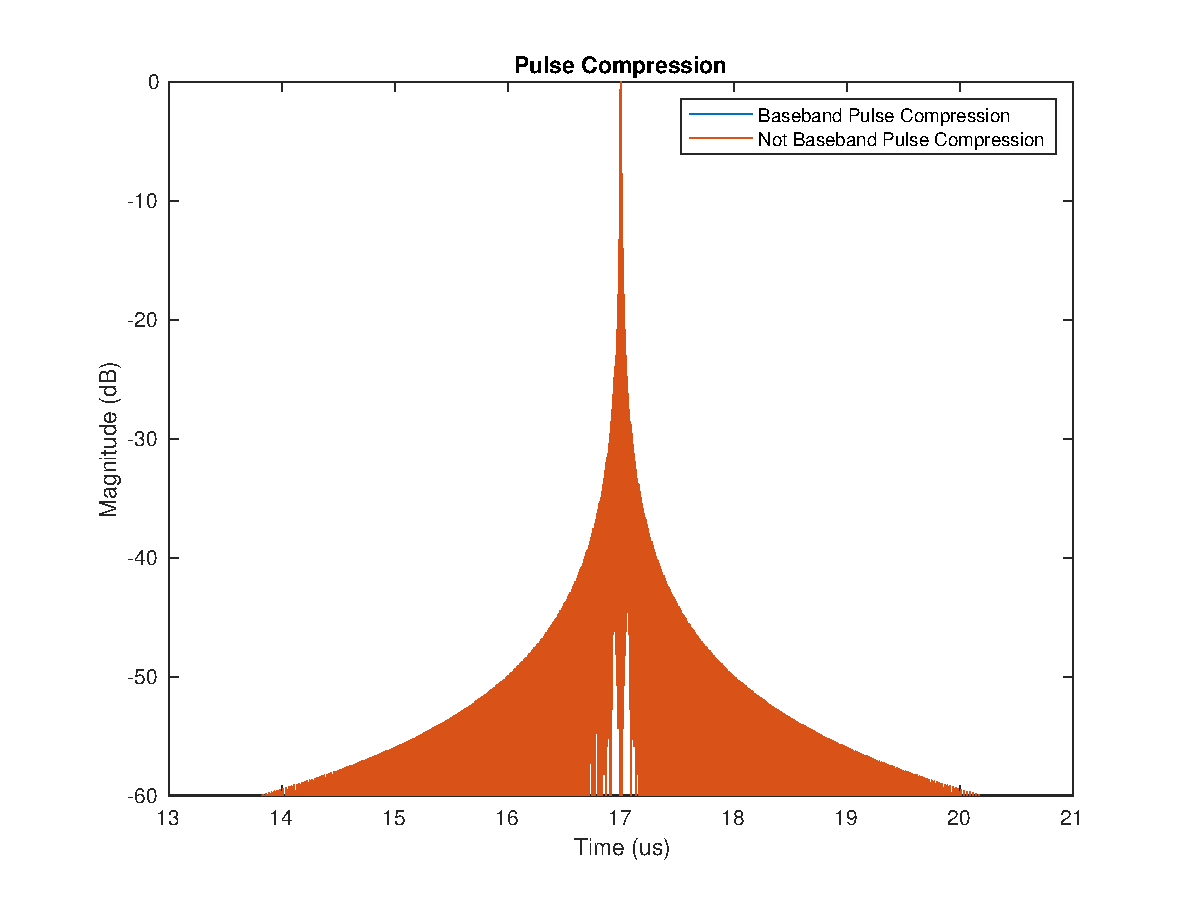
\includegraphics[width=\linewidth]{figure/NotBasebandPulseCompression.eps}
		\caption{非基带信号脉冲压缩结果(功率谱)}
	\end{minipage}
	\begin{minipage}{0.45\linewidth}
		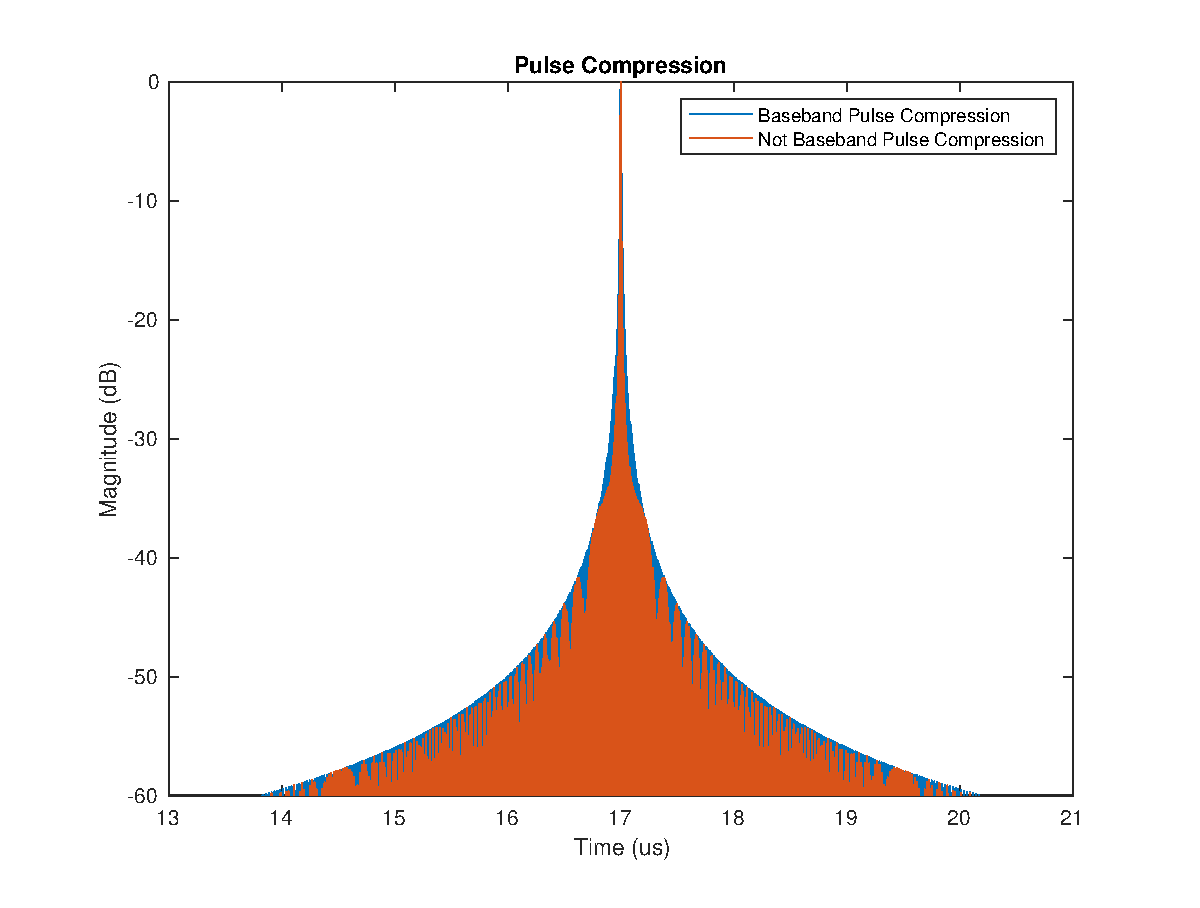
\includegraphics[width=\linewidth]{figure/NotBasebandPulseCompression_real.eps}
		\caption{非基带信号脉冲压缩结果(实部)}
	\end{minipage}
\end{figure}
可以看到非基带脉冲压缩的结果和理论计算结果相同,在功率谱上两者并没有差异。但由于零频率偏移信号中心,所以导致脉冲压缩的结果多了一个相位项,这个相位项就导致了脉冲压缩的结果乘以了一个旋转相位,这一点在脉冲压缩结果的实部上可以明显观察到,非基带信号的脉冲压缩结果的实部乘以了一个频率在信号两侧高、信号中心低的余弦信号。
\subsubsection{加入噪声的脉冲压缩}
在回波信号中加入高斯白噪声,使得回波信号信噪比达到-10dB,进行脉冲压缩,就可以得到如下图所示的脉冲压缩结果。
\singleimage{figure/NoisyPulseCompression.eps}{加入噪声的脉冲压缩}
如上图所示的结果中,可以看到噪声对信号的旁瓣造成了较大影响,使得在信号旁瓣部分能量提高了许多,但对主瓣几乎没有影响。
\subsubsection{加窗后对脉冲压缩}
对匹配滤波器的冲击响应函数加入$\beta=2.5$的Kasier窗进行脉冲压缩,可以得到如下图所示的脉冲压缩结果。
\doubleimages{figure/windowedPulseCompression.eps}{加窗后的脉冲压缩}{figure/windowedPulseCompression_zoomIn.eps}{加窗后的脉冲压缩(放大)}
可以看到加窗后的脉冲压缩的结果的旁瓣能量下降了。将图像放大后进行观察,可以看到副瓣的能量下降了7.68dB,达到了-20.96dB,3dB带宽从原来的$8.8\times 10^{-3}\mu s$展宽至$10.4\times 10^{-3}\mu s$,展宽系数1.18。
\subsubsection{调频率失配的脉冲压缩}
对模拟回波信号的调频率增加$2\%$的差异,进行脉冲压缩可以得到如下图所示的结果。
\singleimage{figure/MissmatchedGammaPulseCompression.eps}{调频率失配的脉冲压缩}
从图中可以看到,调频率的失配对脉冲压缩的结果影响非常大,它引发了主瓣的严重展宽,主瓣能量下降,这不仅对脉冲雷达的测距精度具有非常大的影响,同时对雷达的抗干扰性能、测距范围都具有很严重的不良影响。